\documentclass[xcolor=pdflatex,dvipsnames,table]{beamer}
\usepackage{epsfig,graphicx}
\usepackage{palatino}
\usepackage{fancybox}
\usepackage{relsize}
\usepackage[procnames]{listings}
\usepackage{hyperref}
\usepackage{qtree} % needed?
\usepackage{booktabs}
\usepackage{dirtree}
\usepackage[normalem]{ulem}


% fatter TT font
\renewcommand*\ttdefault{txtt}
% another TT, suggested by Alex
% \usepackage{inconsolata}
% \usepackage[T1]{fontenc} % needed as well?


\newcommand{\scale}{0.7}

\newcommand{\todo}[1]{{\emph{TODO: #1}}}
\newcommand{\martin}[1]{{\color{blue} Martin: #1}}
\newcommand{\abcdef}[1]{{\color{red} Author2: #1}}

% uncomment following for final submission
%\renewcommand{\todo}[1]{}
%\renewcommand{\martin}[1]{}
%\renewcommand{\author2}[1]{}

\newcommand{\code}[1]{{\texttt{#1}}}

\hypersetup{
  linkcolor  = black,
%  citecolor  = blue,
  urlcolor   = blue,
  colorlinks = true,
}

\beamertemplatenavigationsymbolsempty
\setbeamertemplate{footline}[frame number]





\newif\ifbook
% shared in slides and book

\lstdefinelanguage{chisel}{
%  morekeywords={abstract,case,catch,class,def,%
%    do,else,extends,false,final,finally,%
%    for,if,implicit,import,match,mixin,%
%    new,null,object,override,package,%
%    private,protected,requires,return,sealed,%
%    super,this,throw,trait,true,try,%
%    type,val,var,while,with,yield},
%  otherkeywords={=>,<-,<\%,<:,>:,\#,@},
  sensitive=true,
  morecomment=[l]{//},
  morecomment=[n]{/*}{*/},
  morestring=[b]",
  morestring=[b]',
  morestring=[b]"""
}

\usepackage{color}
\definecolor{dkgreen}{rgb}{0,0.6,0}
\definecolor{gray}{rgb}{0.5,0.5,0.5}
\definecolor{mauve}{rgb}{0.58,0,0.82}

% Default settings for code listings
%\ifbook
\lstset{%frame=lines,
  language=chisel,
  aboveskip=3mm,
  belowskip=3mm,
  showstringspaces=false,
  columns=fixed, % basewidth=\mybasewidth,
  basicstyle={\small\ttfamily},
  numbers=none,
  numberstyle=\footnotesize,
  % identifierstyle=\color{red},
  breaklines=true,
  breakatwhitespace=true,
  procnamekeys={def, val, var, class, trait, object, extends},
  % procnamestyle=\ttfamily,
  tabsize=2,
  float
}
%\else
%\lstset{%frame=lines,
%  language=chisel,
%  aboveskip=3mm,
%  belowskip=3mm,
%  showstringspaces=false,
%  columns=fixed, % basewidth=\mybasewidth,
%  basicstyle={\small\ttfamily},
%  numbers=none,
%  numberstyle=\footnotesize\color{gray},
%  % identifierstyle=\color{red},
%  keywordstyle=\color{blue},
%  commentstyle=\color{dkgreen},
%  stringstyle=\color{mauve},
%  breaklines=true,
%  breakatwhitespace=true,
%  procnamekeys={def, val, var, class, trait, object, extends},
%  procnamestyle=\ttfamily\color{red},
%  tabsize=2,
%  float
%}
%\fi

\lstnewenvironment{chisel}[1][]
{\lstset{language=chisel,#1}}
{}

\newcommand{\shortlist}[1]{{\lstinputlisting[nolol]{#1}}}

\newcommand{\longlist}[3]{{\lstinputlisting[float, caption={#2}, label={#3}, frame=tb, captionpos=b]{#1}}}

\newcommand{\verylonglist}[3]{{\lstinputlisting[caption={#2}, label={#3}, frame=tb, captionpos=b]{#1}}}


\title{Testing and Verification}
\author{Martin Schoeberl}
\date{\today}
\institute{Technical University of Denmark\\
Embedded Systems Engineering}

\begin{document}

\begin{frame}
\titlepage
\end{frame}

\begin{frame}[fragile]{Overview}
\begin{itemize}
\item Thomas Aakjer presents digital design at Microchip
\item Review components
\item Debugging and testing
\item Digital designers (sometimes) call testing verification
\begin{itemize}
\item To distinguish from final chip testing
\end{itemize}
\end{itemize}
\end{frame}

\begin{frame}[fragile]{DTU Chip Day}
\begin{itemize}
\item Note the date: Tu 19 April afternoon
\item Start with sandwiches and finish with beer
\item Presentation of chip design and verification work/companies in Denmark
\item The first open-source chip from DTU
\item Several chip companies will present and are prticipating
\item Opportunity to network for: theses with companies, internship, student jobs
\end{itemize}
\end{frame}

%\begin{frame}[fragile]{Some Clarification - TODO: Maybe drop or change}
%\begin{itemize}
%\item Online learning is hard, I understand
%\item Installing all tools on your laptop can also be hard
%\begin{itemize}
%\item We are back physical now
%\end{itemize}
%\item Don't be afraid from the \emph{power user} demos
%\begin{itemize}
%\item Just for ``entertainment'' and for advanced users
%\item You can also simply ignore it
%\end{itemize}
%\item Learning Objectives
%\begin{itemize}
%\item How to build medium sized digital circuits
%\item Describe them in Chisel  and implement them in an FPGA
%\item Timing analysis of digital circuits
%\end{itemize}
%\end{itemize}
%\end{frame}

\begin{frame}[fragile]{Last Chisel Lab (week 3)}
\begin{itemize}
\item On components and small sequential circuits
\begin{itemize}
\item Registers plus combinational circuits
\end{itemize}
\item Did you finish the exercises?
\begin{itemize}
\item Do the poll
\end{itemize}
\item They are not mandatory, but helpful for preparation for the final project
\item Let's look at solutions
\end{itemize}
\end{frame}

\begin{frame}[fragile]{Components are Modules}
\begin{itemize}
\item Components are building blocks
\begin{itemize}
\item Like concrete, physical ICs
\end{itemize}
\item Components have input and output ports (= pins)
\begin{itemize}
\item Organized as a \code{Bundle}
\item assigned to field \code{io}
\end{itemize}
\item We build circuits as a hierarchy of components
\begin{itemize}
\item You did a 4:1 multiplexer out of three 2:1 mulitplexers
\end{itemize}
\item In Chisel a component is called \code{Module}
\item Components/Modules are used to organize the circuit
\begin{itemize}
\item Similar to using methods in Java
\item But they are connected with \emph{wires}
\end{itemize}
\end{itemize}
\end{frame}


\begin{frame}[fragile]{A Binary Watch}
\begin{itemize}
\item Built out of discrete, digital components
\end{itemize}
\begin{figure}
    \centering
    \href{https://commons.wikimedia.org/wiki/File:Relogio_binario.JPG}{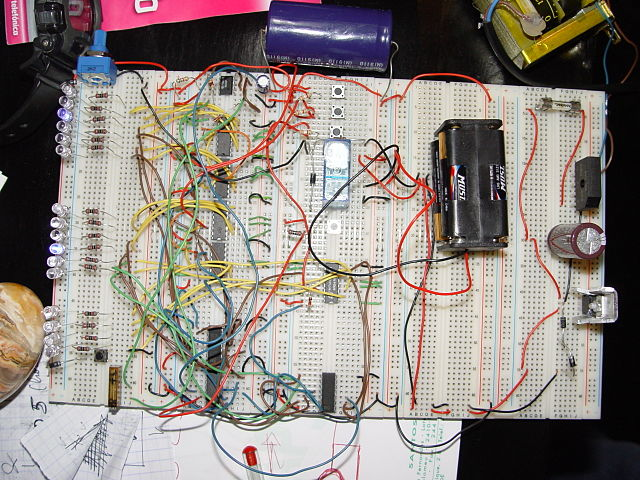
\includegraphics[scale=0.3]{binary-watch.jpg}}
\end{figure}

{\tiny Source: Diogo Sousa, \href{https://en.wikipedia.org/wiki/Public_domain}{public domain}}
\end{frame}


\begin{frame}[fragile]{Let Us Build a Counter}
\begin{itemize}
\item Counting from 0 up to 9
\item Restart from 0
\item Build it out of components
\item We need:
\begin{itemize}
\item Adder
\item Register
\item Multiplexer
\end{itemize}
\item
\item But these are very tiny components
\end{itemize}
\end{frame}

\begin{frame}[fragile]{An Adder (Component/Module)}
\begin{columns}
\begin{column}{0.4\textwidth}
\begin{figure}
  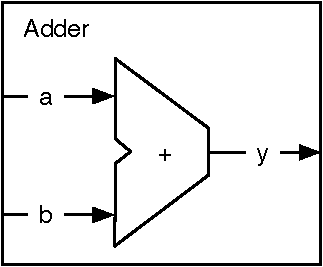
\includegraphics[scale=\scale]{../figures/components-adder}
\end{figure}
\end{column}
\begin{column}{0.6\textwidth}
\shortlist{../code/components_add.txt}
\end{column}
\end{columns}
\end{frame}

\begin{frame}[fragile]{A Register}
\begin{columns}
\begin{column}{0.4\textwidth}
\begin{figure}
  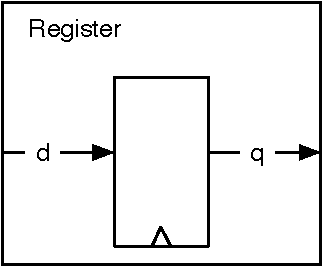
\includegraphics[scale=\scale]{../figures/components-register}
\end{figure}
\end{column}
\begin{column}{0.6\textwidth}
\shortlist{../code/components_reg.txt}
\end{column}
\end{columns}
\end{frame}

\begin{frame}[fragile]{The Counter Schematics}
\begin{figure}
  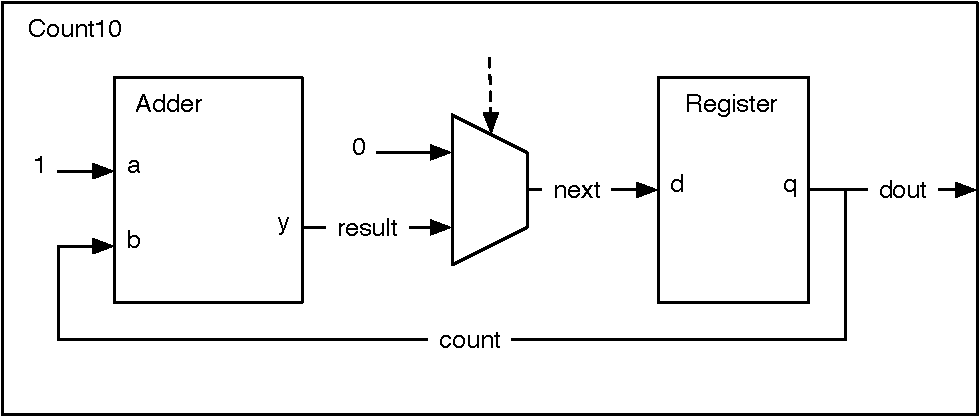
\includegraphics[scale=0.6]{../figures/components-counter}
\end{figure}
\end{frame}

\begin{frame}[fragile]{The Counter in Chisel}
\shortlist{../code/components_cnt.txt}
\end{frame}

\begin{frame}[fragile]{Summarize Components}
\begin{itemize}
\item Think like concrete components (ICs)
\item They have named pins (\code{io.name})
\begin{itemize}
\item In hardware language these pins are often called ports
\item Ports have a direction (input or output)
\end{itemize}
\item They need to be created:
\begin{itemize}
\item \code{val mc = Module(new MyComponent())}
\end{itemize}
\item and pins need to be connected with \code{:=}
\item One module is special, as it is the top model
\end{itemize}
\end{frame}

%\begin{frame}[fragile]{XXX}
%\begin{itemize}
%\item xxx
%\item xxx
%\item xxx
%\item xxx
%\item xxx
%\end{itemize}
%\end{frame}



\begin{frame}[fragile]{Chisel Main}

\begin{itemize}
\item Create one top-level Module
\item Invoke the \code{emitVerilog()} from the App
\item Pass the top module (e.g., \code{new Hello()})
\item Optional: pass some parameters (in an \code{Array})
\item Following code generates Verilog code for the \emph{Hello World}
\end{itemize}
\shortlist{../code/generate.txt}
\end{frame}

\begin{frame}[fragile]{Testing and Debugging}
\begin{itemize}
\item Nobody writes perfect code ;-)
\item We need a method to improve the code
\item In Java we can simply print the result:
\begin{itemize}
\item \code{println("42");}
\end{itemize}
\item What can we do in hardware?
\begin{itemize}
\item Describe the whole circuit and hope it works?
\item We can switch an LED on or off
\end{itemize}
\item We need some tools for \href{https://en.wikipedia.org/wiki/Debugging#/media/File:H96566k.jpg}{debugging}
\item Writing testers in Chisel
\end{itemize}
\end{frame}

\begin{frame}[fragile]{ScalaTest}
\begin{itemize}
\item Testing framework for Scala and Java
\item Tests are placed under \code{src/test/scala}
\item \code{sbt} understands ScalaTest
\item Run all tests with:
\begin{chisel}
sbt test
\end{chisel}
\item When all (unit) tests are ok, the test passes
\item A little bit funny syntax
\item ChiselTest is based on ScalaTest
\end{itemize}
\end{frame}

\begin{frame}[fragile]{Testing with Chisel}
\begin{itemize}
\item A test contains:
\begin{itemize}
\item a device under test (DUT) and
\item the testing logic
\end{itemize}
\item Set input values with \code{poke}
\item Advance the simulation with \code{step}
\item Read the output values with \code{peek}
\item Compare the values with \code{expect}
\item Import following packages:
\shortlist{../code/test_import.txt}
\end{itemize}
\end{frame}

\begin{frame}[fragile]{An Example DUT}
\begin{itemize}
\item A device-under test (DUT)
\item Just 2-bit AND logic
\shortlist{../code/test_dut.txt}
\end{itemize}
\end{frame}

\begin{frame}[fragile]{A ChiselTest}
\begin{itemize}
\item Extends class \code{AnyFlatSpec} with \code{ChiselScalatestTester}
\item Has the device-under test (DUT) as parameter of the \code{test} function
\item Test function contains the test code
\item Testing code can use all features of Scala
\item Is placed in \code{src/test/scala}
\item Is run with: \code{sbt test}
\end{itemize}
\end{frame}

\begin{frame}[fragile]{A Simple Tester}
\begin{itemize}
\item Just using \code{println} for manual inspection
\shortlist{../code/test_bench_simple.txt}
\end{itemize}
\end{frame}


\begin{frame}[fragile]{A Real Tester}
\begin{itemize}
\item Poke values and \code{expect} some output
\shortlist{../code/test_bench.txt}
\end{itemize}
\end{frame}



\begin{frame}[fragile]{Generating Waveforms}
\begin{itemize}
\item Waveforms are timing diagrams
\item Good to see many parallel signals and registers
\begin{verbatim}
sbt "testOnly SimpleTest -- -DwriteVcd=1"
\end{verbatim}
\item Or as additional parameters to test:
\begin{chisel}
test(new DeviceUnderTest)
.withAnnotations(Seq(WriteVcdAnnotation))
\end{chisel}
\item IO signals and registers are dumped
\item Option \code{--debug} puts all wires into the dump
\item Generates a .vcd file
\item Viewing with GTKWave or ModelSim
\end{itemize}
\end{frame}

\begin{frame}[fragile]{Waveform Testing Demo}
\begin{itemize}
\item Counter with a limit from last Chisel lab (\code{Count6})
\item Show Count6 tester: the original and the waveform
\item Run it and look at waveform
\item Add the solution
\item Run again and reload the waveform
\end{itemize}
\end{frame}

\begin{frame}[fragile]{A Self-Running Circuit}
\begin{itemize}
\item \code{Count6} is a self-running circuit
\item Needs no stimuli (\code{poke})
\item Just run for a few cycles
\end{itemize}
\begin{chisel}
    test(new Count6) { dut =>
      dut.clock.step(20)
    }
\end{chisel}
\end{frame}

\begin{frame}[fragile]{The WaveForm}
\begin{itemize}
\item The complete test
\item Note \code{.withAnnotations(Seq(WriteVcdAnnotation)}
\end{itemize}
\begin{chisel}
class Count6WaveSpec extends AnyFlatSpec with ChiselScalatestTester {
  "CountWave6 " should "pass" in {
    test(new Count6).withAnnotations(Seq(WriteVcdAnnotation)) { dut =>
      dut.clock.step(20)
    }
  }
}
\end{chisel}
\end{frame}

\begin{frame}[fragile]{Vending Machine Testing}
\begin{itemize}
\item I provide a minimal tester to generate a waveform
\item Adding some coins and buying
\item You can and shall extend this tester
\item Better having more than one tester
\item Show the waveform of the test
\end{itemize}
\end{frame}


\begin{frame}[fragile]{Printf Debugging}
\begin{itemize}
\item We can \emph{print} in the hardware
\item Printing happens on the rising edge of the clock
\item Good to see many parallel signals and registers
\item \code{printf} anywhere in the module definition
\end{itemize}
\shortlist{../code/test_dut_printf.txt}
\end{frame}


\begin{frame}[fragile]{Test Driven Development (TDD)}
\begin{itemize}
\item Software development process
\begin{itemize}
\item Can we learn from SW development for HW design?
\end{itemize}
\item Writing the test first, then the implementation
\item Started with extreme programming
\begin{itemize}
\item Frequent releases
\item Accept change as part of the development
\end{itemize}
\item A path to \emph{Agile Hardware Development!}
\item Not used in its pour form
\begin{itemize}
\item Writing all those tests is simply considerer too much work
\end{itemize}
\end{itemize}
\end{frame}

\begin{frame}[fragile]{Regression Tests}
\begin{itemize}
\item But tests are collected over time
\item When a bug is found, a test is written to reproduce this bug
\item Collection of tests increases
\item Runs every night to test for \emph{regression}
\begin{itemize}
\item Did a code change introduce a bug in the current code base?
\end{itemize}
\end{itemize}
\end{frame}


\begin{frame}[fragile]{Continuous Integration (CI)}
\begin{itemize}
\item Next logical step from regression tests
\item Run all tests whenever code is changed
\item Automate this with a repository, e.g., on GitHub
\item Run CI on GitHub (moved from Travis yesterday)
\item Show about this on the Chisel book
\begin{itemize}
\item Show \code{sbt test}
\item Live demo on GitHub
\item Mail from GitHub when it fails
\end{itemize}
\item \url{https://github.com/schoeberl/chisel-book/actions}
\item Maybe show how to set this up (it is easy ;)
\begin{itemize}
\item Start with \href{https://github.com/schoeberl/chisel-empty}{chisel-empty} template
\item Open with IntelliJ
\item Add action in GitHub
\end{itemize}
\end{itemize}
\end{frame}

\begin{frame}[fragile]{Continuous Integration}
\begin{itemize}
\item Run your tests on each change
\item Do it also when using source control
\item GitHub Actions (or Trevis)
\item I am doing it even for the Chisel book
\end{itemize}
\end{frame}

\begin{frame}[fragile]{Testing versus Debugging}
\begin{itemize}
\item Debugging is during code development
\item Waveform and \code{println} are easy tools for debugging
\item Debugging does not help for regression tests
\item Write small test cases for regression tests
\item Keeps your code base \emph{intact} when doing changes
\item Better confidence in changes not introducing new bugs
\end{itemize}
\end{frame}


\begin{frame}[fragile]{Scala Build Tool (sbt)}
\begin{itemize}
\item Downloads Scala compiler if needed
\item Downloads dependent libraries (e.g., Chisel)
\item Compiles Scala programs
\item Executes Scala programs
\item Does a lot of magic, maybe too much
\item Compile and run with:
\end{itemize}
\begin{chisel}
sbt "runMain simple.Example"
sbt run
sbt test
sbt "testOnly MySpec"
sbt compile
\end{chisel}
\end{frame}

\begin{frame}[fragile]{Build Configuration - UPDATE!}
\begin{itemize}
\item Defines needed Scala version
\item Library dependencies
\item File name: \code{build.sbt}
\end{itemize}
\begin{chisel}
scalaVersion := "2.12.12"

scalacOptions := Seq("-deprecation", "-Xsource:2.11")

resolvers ++= Seq(
  Resolver.sonatypeRepo("snapshots"),
  Resolver.sonatypeRepo("releases")
)

libraryDependencies += "edu.berkeley.cs" %% "chisel-iotesters" % "1.5.1"
// Chisel 3.4.1 is loaded as a dependency on the tester
\end{chisel}
\end{frame}

\begin{frame}[fragile]{Today's Lab - UPDATE}
\begin{itemize}
\item xxx
\item Show and discuss your testing code with a TA (or me)
\item \href{https://github.com/schoeberl/chisel-lab/tree/master/lab5}{Lab 5}
\end{itemize}
\end{frame}

\begin{frame}[fragile]{Summary}
\begin{itemize}
\item Small sequential circuits are our building blocks
\item We build larger circuits by combining components (modules)
\item There is no \emph{println} in (real) hardware
\item We need to write tests for the development
\item Debugging versus regression tests
\end{itemize}
\end{frame}

\end{document}

